\documentclass[a4paper]{oblivoir}
\usepackage{amsmath,amssymb,kotex,kswrapfig,mdframed,paralist,graphicx,tabu}
\usepackage{fapapersize}
%\usefapapersize{210mm,297mm,10mm,*,10mm,*}

\usepackage{tabto,pifont}
%\TabPositions{0.1\textwidth,0.2\textwidth,0.3\textwidth,0.4\textwidth}
\newcommand\taba[5]{\par\noindent
\ding{172}\:{\ensuremath{#1}}
\tabto{0.2\textwidth}\ding{173}\:\:{\ensuremath{#2}}
\tabto{0.4\textwidth}\ding{174}\:\:{\ensuremath{#3}}
\tabto{0.6\textwidth}\ding{175}\:\:{\ensuremath{#4}}
\tabto{0.8\textwidth}\ding{176}\:\:{\ensuremath{#5}}}

\newcommand\tabb[5]{\par\bigskip\noindent
\ding{172}\:\:{\ensuremath{#1}}
\tabto{0.33\textwidth}\ding{173}\:\:{\ensuremath{#2}}
\tabto{0.66\textwidth}\ding{174}\:\:{\ensuremath{#3}}\medskip\par\noindent
\ding{175}\:\:{\ensuremath{#4}}
\tabto{0.33\textwidth}\ding{176}\:\:{\ensuremath{#5}}}

\newcommand\tabc[5]{\par\bigskip\noindent
\ding{172}\:\:{\ensuremath{#1}}
\tabto{0.5\textwidth}\ding{173}\:\:{\ensuremath{#2}}\medskip\par\noindent
\ding{174}\:\:{\ensuremath{#3}}
\tabto{0.5\textwidth}\ding{175}\:\:{\ensuremath{#4}}\medskip\par\noindent
\ding{176}\:\:{\ensuremath{#5}}}

\newcommand\tabd[5]{\par\bigskip\noindent
\ding{172}\:{\ensuremath{#1}}\medskip\par\noindent
\ding{173}\:\:{\ensuremath{#2}}\medskip\par\noindent
\ding{174}\:\:{\ensuremath{#3}}\medskip\par\noindent
\ding{175}\:\:{\ensuremath{#4}}\medskip\par\noindent
\ding{176}\:\:{\ensuremath{#5}}}

%
\newcommand\one{\ding{172}}
\newcommand\two{\ding{173}}
\newcommand\three{\ding{174}}
\newcommand\four{\ding{175}}
\newcommand\five{\ding{176}}


%\pagestyle{empty}

%%% Counters
\newcounter{num}
%\newcounter{answer}

%%% Commands
\newcommand\prob[1]
{\vs\par\noindent\refstepcounter{num} \textbf{문제 \thenum) #1}\label{#1}\par\noindent}

\newcommand\exam[1]
{\vs\par\noindent\refstepcounter{num} \textbf{예제 \thenum) #1}\par\noindent}

\newenvironment{expl}{\begin{mdframed}[frametitle=풀이]}{\end{mdframed}}

\newcommand\pb[1]{\ensuremath{\fbox{\phantom{#1}}}}

\newcommand\vs[1]{\vspace{50pt}}

\newcommand\an[1]{\par\bigskip\noindent\textbf{문제 \ref{#1})}\\}

\newcommand\ov[1]{\ensuremath{\overline{#1}}}

\newcommand\com[2]{\ensuremath{_{#1}C_{#2}}}

%%% Meta Commands
\let\oldsection\section
\renewcommand\section{\clearpage\oldsection}

\let\emph\textsf

\begin{document}
\title{수지 : 2018-1 기말고사 대비, 수능특강 4--7단원}
\date{\today}
\author{}
\maketitle

%%%
\section{유제}

%
\prob{45-1}%1
주사위를 한 번 던지는 시행에서 나오는 눈의 수의 표본공간을 \(S\)라고 하자.\\
주사위를 한 번 던져서 나온 눈의 수가 \(3\)의 배수인 사건을 \(A\)라고 할 때, \(S\)의 부분집합인 사건 \(B\)가 다음 조건을 만족시킨다.
\begin{mdframed}\begin{enumerate}[(가)]
\item
두 사건 \(A\), \(B\)는 서로 배반사건이다.
\item
\(n(B)=3\)
\end{enumerate}\end{mdframed}
사건 \(B\)의 모든 원소의 합을 \(k\)라고 할 때, \(k\)의 최댓값을 구하시오.
\taba{11}{12}{13}{14}{15}

%
\prob{45-2}
주머니에 \(1\)부터 \(10\)까지의 숫자가 적힌 구슬 열 개가 들어있다.
이 주머니에서 임의로 한 개의 구슬을 고를 때 나오는 눈의 수의 표본공간을 \(S\)라고 하자.
구슬을 골라서 나온 수가 소수인 사건을 \(A\)라고 할 때, \(S\)의 부분집합인 사건 \(B\)가 다음 조건을 만족시킨다.
\begin{mdframed}\begin{enumerate}[(가)]
\item
두 사건 \(A\), \(B\)는 서로 배반사건이다.
\item
\(n(B)=2\)
\end{enumerate}\end{mdframed}
사건 \(B\)의 모든 원소의 합을 \(k\)라고 할 때, \(k\)의 최솟값을 구하시오.
\taba34567

\newpage
%
\prob{47-1}%5
한 개의 주사위를 \(2\)번 던져서 나오는 눈의 수를 차례로 \(a\), \(b\)라 할 때,\\ \((-1)^a+(-1)^b=0\)일 확률을 \(p\)라고 하자.
\(72p\)의 값을 구하시오.
\taba{20}{24}{28}{32}{36}

%
\prob{47-2}%1
한 개의 주사위를 \(2\)번 던져서 나오는 눈의 수를 차례로 \(a\), \(b\)라 할 때,\\ \(i^{a+1}+i^{b-1}=0\)일 확률을 \(p\)라고 하자.
\(72p\)의 값을 구하시오.
\taba{20}{24}{28}{32}{36}

%
\prob{49-1}%1
\(5\)장의 카드\:\: \fbox0,\:\:\fbox1, \:\:\fbox2, \:\:\fbox3, \:\:\fbox4 중에서 임의로 서로 다른 \(3\)장의 카드를 뽑아 일렬로 나열하여 세 자리 자연수를 만들 때, 그 자연수가 \(4\)의 배수 혹은 \(5\)의 배수가 될 확률을 \(p\)라고 하자.
\(240p\)의 값을 구하시오.
\taba{105}{126}{144}{168}{208}

%
\prob{49-2}%3
\(5\)장의 카드\:\: \fbox1, \:\:\fbox2, \:\:\fbox3, \:\:\fbox4, \:\:\fbox5 중에서 임의로 서로 다른 \(3\)장의 카드를 뽑아 일렬로 나열하여 세 자리 자연수를 만들 때, 그 자연수가 \(2\)의 배수 혹은 \(5\)의 배수가 될 확률을 \(p\)라고 하자.
\(240p\)의 값을 구하시오.
\taba{105}{126}{144}{168}{208}

%
\prob{49-3}%5
\(5\)장의 카드\:\: \fbox1, \:\:\fbox2, \:\:\fbox3, \:\:\fbox4, \:\:\fbox5 중에서 임의로 서로 다른 \(3\)장의 카드를 뽑아 일렬로 나열하여 세 자리 자연수를 만들 때, 그 자연수가 \(2\)의 배수 혹은 \(3\)의 배수가 될 확률을 \(p\)라고 하자.
\(240p\)의 값을 구하시오.
\taba{105}{126}{144}{168}{208}

\newpage
%
\prob{51-1}%3%a=7
어느 학급의 전체 학생 \(34\)명을 대상으로 방과후학교 수업을 희망하는 학생의 수를 국어, 영어, 수학 과목에 대하여 조사하였다.
두 과목을 이상을 희망하는 학생은 \(a\)명이고, 한 과목도 희망하지 않는 학생은 \(9\)명이었다.
이 학급의 학생 중에서 임의로 1명을 선택할 때, 이 학생이 방과후학교 수업을 한 과목만 희망할 학생일 확률은 \(\frac9{17}\)이다.
\(a\)의 값은?
\taba56789

%
\prob{51-2}%1%a=5
어느 학급의 전체 학생 \(30\)명을 대상으로 방과후학교 수업을 희망하는 학생의 수를 영어, 수학 과목에 대하여 조사하였다.
두 과목을 희망하는 학생은 \(a\)명이고, 한 과목도 희망하지 않는 학생은 \(12\)명이었다.
이 학급의 학생 중에서 임의로 1명을 선택할 때, 이 학생이 방과후학교 수업을 한 과목만 희망할 학생일 확률은 \(\frac{13}{30}\)이다.
\(a\)의 값은?
\taba56789

%
\prob{57-1}%3
어느 학교의 전체 학생 \(200\)명 중에서 스마트폰을 가지고 있는 여학생은 \(60\)명이고, 스마트폰을 가지고 있지 않은 학생은 \(75\)명이다.
이 학교의 학생 중에서 임의로 선택한 1명이 스마트폰을 가지고 있는 학생일 때, 이 학생이 남학생일 확률은?
\taba{\frac{11}{25}}{\frac{12}{25}}{\frac{13}{25}}{\frac{14}{25}}{\frac45}

%
\prob{57-2}%3
어느 학교의 전체 학생 \(320\)명 중에서 안경을 쓴 남학생은 \(153\)명이고, 전체 여학생의 수는 \(140\)명이다.
이 학교의 학생 중에서 임의로 선택한 1명이 남학생일 때, 이 학생이 안경을 쓰지 않았을 확률은?
\taba{\frac1{20}}{\frac1{10}}{\frac3{20}}{\frac15}{\frac14}

\newpage
%
\prob{57-3}%3
어느 학교의 전체 학생은 \(360\)명이고, 각 학생은 체험 학습 \(A\), 체험 학습 \(B\) 중 하나를 선택하였다.
이 학교의 학생 중 체험 학습 \(A\)를 선택한 학생은 남학생 \(90\)명과 여학생 \(70\)명이다.
이 학교의 학생 중 임의로 뽑은 \(1\)명의 학생이 체험 학습 \(B\)를 선택한 학생일 때, 이 학생이 남학생일 확률이 \(\frac25\)이다.
이 학교의 여학생의 수는?
\taba{180}{185}{190}{195}{200}

%
\prob{59-1}%5
프리미어 리그 \(T\)팀에서 활약중인 \(S\)선수는 \(3\)번에 \(2\)번 꼴로 경기에 출전한다.
\(S\)선수가 출전한 경기에서 \(T\)팀이 승리할 확률은 \(70\%\)이고, \(S\)선수가 출전하지 않은 경기에서 \(T\)팀이 승리하지 못할 확률은 \(40\%\)이다.
\(T\)팀이 치른 전체 경기에서 임의로 선택한 한 경기가 \(T\)팀이 승리한 경기일 때, 이 경기가 \(S\)선수가 출전한 경기일 확률은?
\taba{\frac12}{\frac{11}{20}}{\frac35}{\frac{13}{20}}{\frac7{10}}

%
\prob{59-2}%4
월드컵에 출전한 \(P\)팀에서 활약중인 \(R\) 선수는 \(4\)번에 \(3\)번 꼴로 경기에 출전한다.
\(R\) 선수가 출전한 경기에서 \(P\)팀이 승리할 확률은 \(\frac45\)이고, \(R\)선수가 출전하지 않은 경기에서 \(P\)팀이 승리할 확률은 \(\frac25\)이다.
\(P\)팀이 치른 전체 경기에서 임의로 선택한 한 경기가 \(P\)팀이 승리한 경기일 때, 이 경기가 \(R\)선수가 출전한 경기일 확률은?
\taba{\frac9{14}}{\frac57}{\frac{11}{14}}{\frac67}{\frac{13}{14}}

%
\prob{61-1}%3
두 사건 \(A\), \(B\)가 독립이고
\[P(A\cap B)=\frac14,\quad P(A^C\cap B)=\frac16\]
일 때, \(P(A)\)의 값은?
(단, \(A^C\)는 \(A\)의 여사건이다.)
\taba{\frac25}{\frac12}{\frac35}{\frac7{10}}{\frac45}

%
\prob{61-2}%5
두 사건 \(A\), \(B\)가 독립이고
\[P(A^C)=\frac34,\quad P(A\cup B^C)=\frac3{10}\]
일 때, \(P(B)\)의 값은?
(단, \(A^C\)는 \(A\)의 여사건이다.)
\taba{\frac23}{\frac{11}{15}}{\frac45}{\frac{13}{15}}{\frac{14}{15}}

%
\prob{63-1}%1
프로야구 한국시리즈에 진출한 두 팀 \(A\), \(B\)는 \(7\)번의 경기 중 먼저 \(4\)번 이기는 팀이 우승을 한다.
\(3\)번의 경기가 끝난 결과 \(A\)팀이 1승 2패로 뒤져 있다.
\(A\)팀이 한 경기에서 \(B\)팀을 이길 확률이 \(\frac34\)일 때, 한국시리즈에서 \(A\)팀이 우승할 확률은?
(단, 비기는 경우는 없다.)
\taba{\frac{189}{256}}{\frac{95}{128}}{\frac{191}{256}}{\frac34}{\frac{193}{256}}

%
\prob{63-2}%1
프로야구 한국시리즈에 진출한 두 팀 \(A\), \(B\)는 \(7\)번의 경기 중 먼저 \(4\)번 이기는 팀이 우승을 한다.
\(3\)번의 경기가 끝난 결과 \(A\)팀이 0승 2패로 뒤져 있다.
\(A\)팀이 한 경기에서 \(B\)팀을 이길 확률이 \(\frac23\)일 때, 한국시리즈에서 \(A\)팀이 우승할 확률은?
(단, 비기는 경우는 없다.)
\taba{\frac{80}{243}}{\frac13}{\frac{82}{243}}{\frac{83}{243}}{\frac{28}{81}}

%
\prob{71-1}%4
확률변수 \(X\)가 갖는 값이 \(1\), \(2\), \(3\)이고, \(X\)의 확률질량함수가
\[P(X=x)=\frac{k\times\com3x}{\com5x}\quad(x=1,2,3)\]
일 때, 상수 \(k\)의 값은?
\taba{\frac12}{\frac23}{\frac56}1{\frac76}

%
\prob{71-2}%5
확률변수 \(X\)가 갖는 값이 \(0\), \(1\), \(2\), \(3\)이고, \(X\)의 확률질량함수가
\[P(X=x)=\frac{k\times\com3x}{\com6{2x}}\quad(x=0,1,2,3)\]
일 때, 상수 \(k\)의 값은?
\taba{\frac1{12}}{\frac16}{\frac14}{\frac13}{\frac5{12}}

%
\prob{73-1}%2
확률변수 \(X\)의 확률분포가 다음과 같을 때, \(\sigma(-5X+3)\)을 구하여라.
\begin{center}
\begin{tabu}to.8\textwidth{X[1.5$c]|X[$c]X[$c]X[$c]X[$c]|X[$c]}
\hline
X		&1			&2			&3				&4			&합계\\\hline
P(X=x)	&\frac1{10}&\frac12	&\frac3{10}	&\frac1{10}&1\\\hline
\end{tabu}
\end{center}
\taba2468{10}

%
\prob{73-2}%2
확률변수 \(X\)의 확률분포가 다음과 같을 때, \(E(aX+10)\)을 구하여라.
\begin{center}
\begin{tabu}to.8\textwidth{X[1.5$c]|X[$c]X[$c]X[$c]|X[$c]}
\hline
X		&200		&300	&500	&합계\\\hline
P(X=x)	&\frac12	&a		&4a^2	&1\\\hline
\end{tabu}
\end{center}
\taba{80}{85}{90}{95}{100}

\newpage
%
\prob{75-1}%5
그림과 같이 좌표 평면 위에 \(x\)좌표와 \(1\) 또는 \(2\) \(y\)좌표가 각각 \(1\) 또는 \(2\)인 \(6\)개의 점이 있다.
이 \(6\)개의 점 중에서 임의로 서로 다른 \(2\)개의 점을 동시에 택할 때, 두 점의 \(x\)좌표의 합을 확률변수 \(X\)라고 하자.
\(V(X)\)의 값을 구하시오.
\begin{center}
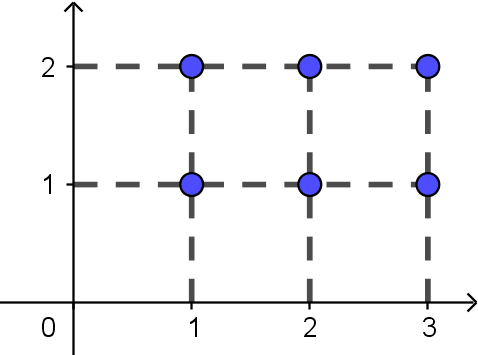
\includegraphics[width=0.3\textwidth]{75_1}
\end{center}
\taba{\frac45}{\frac{13}{15}}{\frac{14}{15}}1{\frac{16}{15}}

%
\prob{75-2}%2
주머니에 \(1\), \(3\), \(5\), \(7\)이 적힌 숫자가 적힌 구슬 네 개가 들어있다.
이 주머니에서 두 개의 구슬을 동시에 꺼냈을 때, 두 구슬에 적힌 숫자들의 합을 \(X\)라고 할 때, \(V(X)\)의 값을 구하여라.
\taba{20}{\frac{20}3}4{\frac{20}7}{\frac{20}9}

%
\prob{77-1}%5
확률변수 \(X\)가 갖는 값이 \(0\), \(1\), \(2\), \(\cdots\), \(18\)이고 \(X\)의 확률질량함수가
\[P(X=x)=\com{18}x\left(\frac23\right)^x\left(\frac13\right)^{18-x}\quad(x=0,1,2,\cdots,18)\]
일 때, \(E(X^2)\)의 값을 구하시오.
\taba{92}{106}{120}{134}{148}

\newpage
%
\prob{77-2}%2
확률변수 \(X\)가 갖는 값이 \(0\), \(1\), \(2\), \(\cdots\), \(25\)이고 \(X\)의 확률질량함수가
\[P(X=x)=\com{25}x\times\frac{2^x\times3^{25-x}}{5^{25}}\quad(x=0,1,2,\cdots,25)\]
일 때, \(E(X^2)\)의 값을 구하시오.
\taba{92}{106}{120}{134}{148}

%
\prob{85-1}%1
연속확률변수 \(X\)가 갖는 값의 범위가 \(0\le X\le 5\)이고, 확률변수 \(X\)의 확률밀도함수 \(y=f(x)\)의 그래프가 그림과 같을 때, \(P(1\le X\le 3)=\frac qp\)이다.
\(p+q\)의 값을 구하여라.
(단, \(a\)는 \(a>0\)인 상수이고 \(p\)와 \(q\)는 서로소인 자연수이다.)
\begin{center}
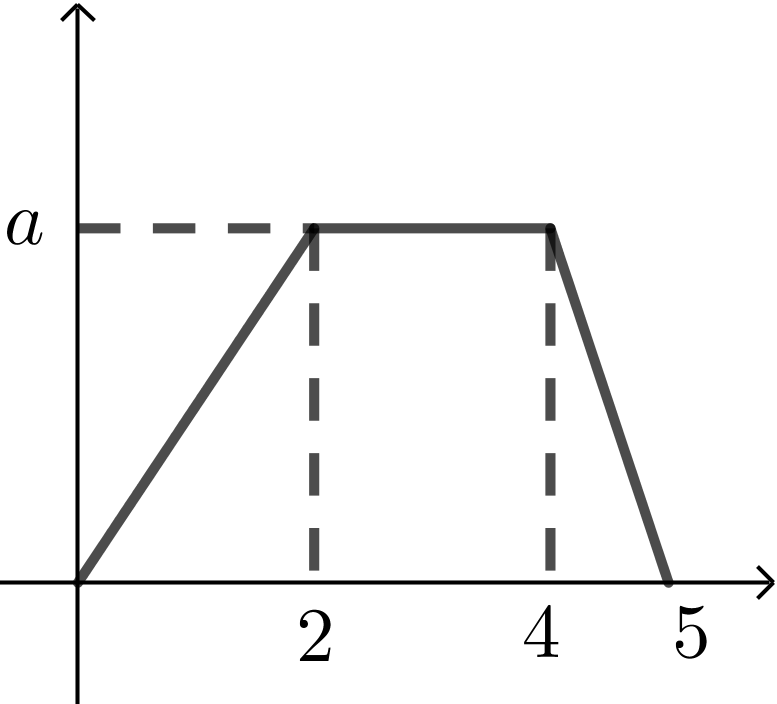
\includegraphics[width=0.3\textwidth]{85_1}
\end{center}
\taba3{13}{23}{33}{43}

%
\prob{85-2}%4
연속확률변수 \(X\)가 갖는 값의 범위가 \(0\le X\le 6\)이고, 확률변수 \(X\)의 확률밀도함수 \(y=f(x)\)의 그래프가 그림과 같을 때, \(P(4\le X\le 5)=\frac qp\)이다.
\(p+q\)의 값을 구하여라.
(단, \(a\)는 \(a>0\)인 상수이고 \(p\)와 \(q\)는 서로소인 자연수이다.)
\begin{center}
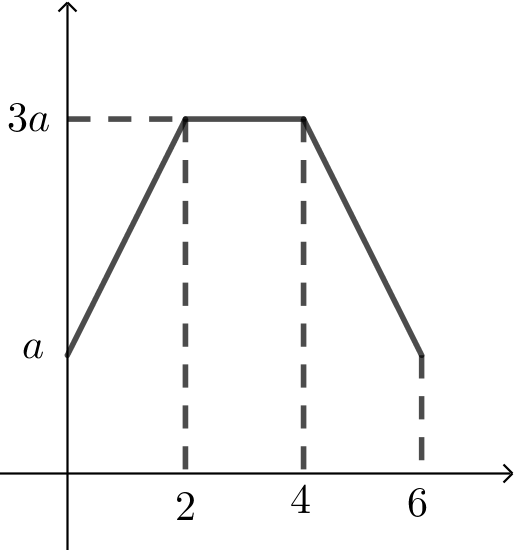
\includegraphics[width=0.3\textwidth]{85_2}
\end{center}
\taba3{13}{23}{33}{43}

%87은 생략

\newpage
%
\prob{89-1}%2
어느 회사에서 국내 본사와 해외 지사에 근무할 신입사원을 각각 선발하였다.
국내 본사 지원자의 입사 시험 성적을 조사하였더니 평균이 \(650\)점, 표준편차가 \(30\)점인 정규분포를 따르고,
해외 지사 지원자의 입사 시험 성적을 조사하였더니 평균이 \(625\)점, 표준편차가 \(40\)점인 정규분포를 따른다고 한다.
국내 본사 지원자 중 임의로 선택한 한 명의 입사 시험 성적이 \(710\)점 이상일 확률을 \(p_1\),
해외 지사 지원자 중 임의로 선택한 한 명의 입사 시험 성적이 \(a\)점 이상일 확률을 \(p_2\)라고 하자.
\(p_1\le p_2\)를 만족시키는 실수 \(a\)의 최댓값은?
\taba{700}{705}{710}{715}{720}

%
\prob{89-2}%3
어떤 고등학교의 \(A\)반과 \(B\)반의 수학 성적을 조사하였다.
\(A\)반의 중간고사 수학 점수은 평균이 \(60\)점, 표준편차가 \(6\)점인 정규분포를 따르고,
\(B\)반의 중간고사 수학 점수은 평균이 \(50\)점, 표준편차가 \(10\)점인 정규분포를 따른다.
\(A\)반에서 임의로 선택한 한 명의 수학 점수가 \(63\)점 이상일 확률을 \(p_1\),
\(B\)반에서 임의로 선택한 한 명의 수학 점수가 \(a\)점 이상일 확률을 \(p_2\)라고 하자.
\(p_1\ge p_2\)를 만족시키는 실수 \(a\)의 최솟값은?
\taba{51}{53}{55}{57}{59}

\newpage
\fbox{다음 표준정규분포표를 사용하여 문제 \ref{91-1})--\ref{91-2})를 풀어라.}
\begin{center}
\begin{tabu}to.4\textwidth{X[1$c]|X[$2c]}
\hline
z	&P(0\le Z\le z)\\\hline
0.5	&0.1915\\\hline
1.0	&0.3413\\\hline
1.5	&0.4332\\\hline
2.0	&0.4772\\\hline
\end{tabu}
\end{center}

%
\prob{91-1}%2%p=4/5
확률변수 \(X\)가 이항분포 \(B(100,p)\)를 따르고 \(E(2X+40)=200\)일 때,\\
\(P(84\le X\le88)\)의 값을 구하여라.
\taba{0.0228}{0.1498}{0.1587}{0.3085}{0.5328}

%
\prob{91-2}%5%n=147
확률변수 \(X\)가 이항분포 \(B(n,\frac37)\)를 따르고 \(\sigma(X)=6\)일 때,\\
\(P(57\le X\le66)\)의 값을 구하여라.
\taba{0.0228}{0.1498}{0.1587}{0.3085}{0.5328}

%%
\section{Level 1 : 기초연습}
%
\prob{52-1}%5
\(1\)부터 \(16\)까지의 자연수가 하나씩 적힌 \(16\)장의 카드 중에서 임의로 한 장의 카드를 뽑을 때, 뽑힌 카드에 적힌 수가 소수인 사건을 \(A\)라고 하고 \(n\) 이상의 자연수인 사건을 \(B_n\)이라고 하자.
두 사건 \(A\), \(B_n\)이 서로 배반사건이 되도록 하는 모든 자연수 \(n\)의 값의 합은?
(단, \(n=1,2,3,\cdots,16\))
\taba{29}{33}{37}{41}{45}

%
\prob{52-2}%1
남학생 \(3\)명, 여학생 \(5\)명 중 임의로 \(3\)명의 임원을 동시에 선택할 때, 남학생과 여학생이 적어도 \(1\)명씩 임원에 포함될 확률은?
(단, 임원은 서로 구별하지 않는다.)
\taba{\frac{45}{56}}{\frac{23}{28}}{\frac{47}{56}}{\frac67}{\frac78}

%
\prob{64-1}%3
어떤 학급의 전체 학생 \(33\)명을 대상으로 줄넘기 시험을 실시하였다.
\(1\)차 줄넘기 시험에 불합격한 학생을 대상으로 \(2\)차 줄넘기 시험을 실시하여 \(1\)차, \(2\)차 줄넘기 시험에서 각각 \(20\)명, \(8\)명의 학생이 합격하였다.
이 학급의 학생 중에서 임의로 선택한 \(1\)명이 줄넘기 시험에서 합격한 시험일 때, 이 학생이 \(2\)차 줄넘기 시험에서 합격한 학생일 확률은?
\taba{\frac17}{\frac3{14}}{\frac27}{\frac5{14}}{\frac37}

%
\prob{64-2}%3
어떤 학생이 대학수학능력시험을 준비하는 \(100\)일 동안, 하루도 빠지지 않고 그날의 공부시간을 체크했다.
\(100\)일 중 공부를 아예 하지 않고 쉰 날이 \(16\)일이고 \(8\)시간 이상 공부한 날이 \(56\)일이다.
\(100\)일 중 임의로 선택한 날이 공부를 한 날일 때, 이날 이 학생이 \(8\)시간 미만으로 공부했을 확률은?
\taba{\frac16}{\frac14}{\frac13}{\frac5{12}}{\frac12}

%
\prob{64-3}%4
한 개의 주사위를 \(2\)번 던지는 시행에서 나오는 눈의 수를 차례로 \(a\), \(b\)라고 할 때, 두 수의 곱 \(ab\)가 짝수일 확률은?
\taba{\frac12}{\frac7{12}}{\frac23}{\frac34}{\frac56}

%
\prob{64-4}%5
한 개의 주사위를 \(3\)번 던지는 시행에서 나오는 눈의 수를 차례로 \(a\), \(b\), \(c\)라고 할 때, 세 수의 곱 \(abc\)가 \(8\)의 배수일 확률은?
\taba{\frac7{24}}{\frac13}{\frac38}{\frac5{12}}{\frac{11}{24}}

%
\prob{78-1}%4
확률변수 \(X\)의 확률분포가 다음과 같다.
\(b=3a\)일 때, 두 상수 \(a\), \(b\)에 대하여 \(ab\)의 값은?
\begin{center}
\begin{tabu}to.8\textwidth{X[1.5$c]|X[$c]X[$c]X[$c]X[$c]|X[$c]}
\hline
X		&0			&1	&2			&3		&합계\\\hline
P(X=x)	&\frac1{12}&a	&\frac14	&b		&1\\\hline
\end{tabu}
\end{center}
\taba{\frac1{18}}{\frac1{16}}{\frac1{14}}{\frac1{12}}{\frac1{10}}

%
\prob{78-2}%1
확률변수 \(X\)의 확률분포가 다음과 같다.
\(E(X)=\frac73\)일 때, 두 상수 \(a\), \(b\)에 대하여 \(b-a\)의 값은?
\begin{center}
\begin{tabu}to.8\textwidth{X[1.5$c]|X[$c]X[$c]X[$c]|X[$c]}
\hline
X		&1	&2	&3			&합계\\\hline
P(X=x)	&a	&b	&\frac12	&1\\\hline
\end{tabu}
\end{center}
\taba{\frac16}{\frac14}{\frac13}{\frac5{12}}{\frac12}

\newpage
%
\prob{79-1}%4
확률변수 \(X\)에 대하여 \(E(2X+4)=12\), \(V(2X)=36\)일 떄, \(E(X^2)\)의 값을 구하여라.
\taba{16}{19}{22}{25}{28}

%
\prob{79-2}%2
서로 다른 2개의 주사위를 동시에 던지는 시행을 \(72\)회 반복할 때, \(2\)개의 주사위를 동시에 던져서 나온 두 눈의 수의 합이 \(5\) 이하인 횟수를 확률변수 \(X\)라고 하자.
\(\sigma(X)\)의 값을 구하시오.
\taba{17}{20}{23}{26}{29}

%
\prob{79-3}%5
서로 다른 2개의 주사위를 동시에 던지는 시행을 \(48\)회 반복할 때, \(2\)개의 주사위를 동시에 던져서 나온 두 눈의 수의 합이 \(4\)의 배수인 횟수를 확률변수 \(X\)라고 하자.
\(\sigma(X)\)의 값을 구하시오.
\taba{\sqrt5}{\sqrt6}{\sqrt7}{2\sqrt2}{3}

%
\prob{92-1}%1
연속확률변수 \(X\)가 갖는 값의 범위가 \(0\le X\le 3\)이고, 확률변수 \(X\)의 확률밀도함수 \(y=f(x)\)의 그래프가 그림과 같을 때, \(P(0\le X\le a)=\frac23\)이다.
두 상수 \(a\), \(b\)에 대하여 \(a-3b\)의 값은?
\begin{center}
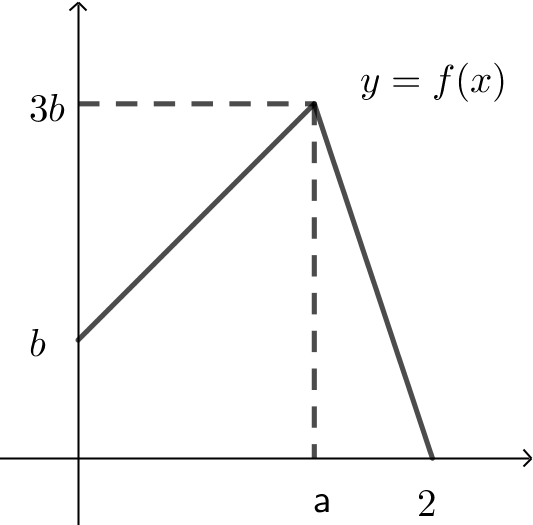
\includegraphics[width=0.4\textwidth]{92_1}
\end{center}
\taba{\frac{61}{30}}{\frac{31}{15}}{\frac{21}{10}}{\frac{32}{15}}{\frac{13}6}

\bigskip\bigskip
\fbox{다음 표준정규분포표를 사용하여 문제 \ref{92-2}--\ref{92-3}를 풀어라.}
\begin{center}
\begin{tabu}to.4\textwidth{X[1$c]|X[$2c]}
\hline
z	&P(0\le Z\le z)\\\hline
0.5	&0.1915\\\hline
1.0	&0.3413\\\hline
1.5	&0.4332\\\hline
2.0	&0.4772\\\hline
\end{tabu}
\end{center}

%
\prob{92-2}%2
서로 다른 \(2\)개의 주사위를 동시에 던져서 나오는 두 눈의 수를 확인하는 시행을 한다.
이 시행을 \(162\)번 반복할 때, 두 눈의 수가 모두 \(3\)의 배수가 나오는 횟수가 \(16\)회 이하일 확률을 구하여라.
\taba{0.0228}{0.0668}{0.1587}{0.3085}{0.4772}

%
\prob{92-3}%4
세 개의 동전을 던지는 시행을 \(192\)회 반복할 때, 세 개의 동전이 모두 같은 면인 횟수가 \(39\)회 이하일 확률을 구하여라.
\taba{0.0228}{0.0668}{0.1587}{0.3085}{0.4772}

%%
\section*{답}

\begin{minipage}{0.2\textwidth}
\an{45-1}\one
\an{45-2}\three
\an{47-1}\five
\an{47-2}\one
\an{49-1}\one
\an{49-2}\three
\an{49-3}\five
\an{51-1}\three
\an{51-2}\one
\an{57-1}\three
\an{57-2}\three
\end{minipage}
\begin{minipage}{0.2\textwidth}
\an{57-3}\three
\an{59-1}\five
\an{59-2}\four
\an{61-1}\three
\an{61-2}\five
\an{63-1}\one
\an{63-2}\one
\an{71-1}\four
\an{71-2}\five
\an{73-1}\two
\an{73-2}\two
\end{minipage}
\begin{minipage}{0.2\textwidth}
\an{75-1}\five
\an{75-2}\two
\an{77-1}\five
\an{77-2}\two
\an{85-1}\one
\an{85-2}\four
\an{89-1}\two
\an{89-2}\three
\an{91-1}\two
\an{91-2}\five
\an{52-1}\five
\an{52-2}\one
\end{minipage}
\begin{minipage}{0.2\textwidth}
\an{64-1}\three
\an{64-2}\three
\an{64-3}\four
\an{64-4}\five
\an{78-1}\four
\an{78-2}\one
\an{79-1}\four
\an{79-2}\two
\an{79-3}\five
\an{92-1}\one
\an{92-2}\two
\an{92-3}\four
\end{minipage}

\end{document}